\section{The squarefree series and the clock}\label{sec:sqfree}

Riesz's criterion (Sections~\ref{wr:sec:riesz} and \ref{ch:riesz}) reads RH from a function whose Mellin transform is $\Gamma(1-s)/\zeta(2s)$. The squarefree integers carry the same reciprocal $1/\zeta(2s)$. Their Dirichlet series is
\begin{equation}\label{eq:sqfree:D}
D(s)=\sum_{n\ge1}\frac{\mu(n)^2}{n^s}=\prod_p\big(1+p^{-s}\big)=\frac{\zeta(s)}{\zeta(2s)},\qquad\re s>1,
\end{equation}
whose singularities in the half plane $\re s>0$ are the pole at $s=1$ and the poles at the points $\rho/2$ at which $\zeta(\rho/2)\ne0$ (all of them under RH), and the number $Q(x)$ of squarefree integers up to $x$ oscillates about $6x/\pi^2$ on the scale $x^{1/4}$ that these poles set when they lie on the line $\re s=\frac14$, that is under RH. This section follows the first author's note \cite{P26sqf}, which starts from a Math StackExchange thread \cite{MSE2063166} on the partial sums of $\mu(n)^2n^{-\alpha}$ over $\mathbb Q$ and over number fields. Write $\Delta(x)=Q(x)-6x/\pi^2$ for the error. The bound $\Delta(x)=O(x^{1/4+\varepsilon})$ is open even under RH, but it is equivalent to RH once the count is smoothed by an exponential or a Gamma(2) law, and in mean square; the order $x^{1/4}$ is attained with no hypothesis; and the bound for the count smoothed by a Gamma($n$) law loses a factor $n^{1/8}$, which still gives $\Delta(x)=O(x^{2/5+\varepsilon})$ under RH (Sections~\ref{sec:sqfree:smooth} and \ref{sec:sqfree:meansq}). The P\'olya kernels of the Dedekind zeta functions of imaginary quadratic fields, whose positivity can fail, are in Section~\ref{sec:sqfree:quad} of Chapter~\ref{chap:probability}.

We keep the notation of Section~\ref{ch:clock} for the P\'olya variable $X$, with $\E e^{sX}=\xi(\frac12+s)/\xi(\frac12)$, the clock $T$, $G(u)=\xi(\frac12+\sqrt u)/\xi(\frac12)$, the numbers $a_k=-(\rho_k-\frac12)^2$, the heat trace $W(t)=\sum_ke^{-a_kt}$ and the measure $U_{\RH}$, and the notation of Section~\ref{bp:sec:mellin} for the tilted variables $V_\alpha$, with $\E e^{sV_\alpha}=\xi(\alpha+s)/\xi(\alpha)$, and $b_\alpha=\frac{\xi'}\xi(\alpha)=\E V_\alpha$. Throughout, $\mu$ is the M\"obius function, $M(t)=\sum_{d\le t}\mu(d)$ is the Mertens function, $\{y\}$ is the fractional part of $y$, and
\[
Q(x)=\sum_{n\le x}\mu(n)^2,\qquad \Delta(x)=Q(x)-\frac6{\pi^2}\,x .
\]

\subsection{The thread: Perron's formula and an elementary method}\label{sec:sqfree:thread}

The question asks for the behaviour as $x\to\infty$ of
\[
S_\alpha(x)=\sum_{N(\mathfrak a)\le x}\frac{\mu(\mathfrak a)^2}{N(\mathfrak a)^\alpha},
\]
the sum running over the integral ideals $\mathfrak a$ of a number field $K$, with $\mu$ the M\"obius function of ideals and $N$ the norm, and, in a comment, for its expansion at $\alpha=1$. Over $\mathbb Q$, $S_\alpha(x)=\sum_{n\le x}\mu(n)^2n^{-\alpha}$, and another comment points to Abel summation from the classical count
\begin{equation}\label{eq:sqfree:Q}
Q(x)=\frac6{\pi^2}\,x+O(\sqrt x).
\end{equation}
The accepted answer applies Perron's formula over $K$, and the other answer carries out the elementary method over $\mathbb Q$. Neither evaluates the constant at $\alpha=1$.

Since $\mu(\mathfrak p^k)^2$ is $1$ for $k\le1$ and $0$ for $k\ge2$, the Euler factor of $\sum_{\mathfrak a}\mu(\mathfrak a)^2N(\mathfrak a)^{-s}$ at a prime ideal $\mathfrak p$ is $1+N(\mathfrak p)^{-s}=(1-N(\mathfrak p)^{-2s})/(1-N(\mathfrak p)^{-s})$, so the series is $\zeta_K(s)/\zeta_K(2s)$, with $\zeta_K$ the Dedekind zeta function of $K$, and
\begin{equation}\label{eq:sqfree:perron}
S_\alpha(x)=\frac1{2\pi i}\int_{\sigma-i\infty}^{\sigma+i\infty}\frac{\zeta_K(\alpha+s)}{\zeta_K(2\alpha+2s)}\,x^s\,\frac{ds}s,\qquad \sigma>\max\{1-\alpha,0\}.
\end{equation}

The integrand of \eqref{eq:sqfree:perron} has a simple pole at $s=1-\alpha$, a pole at $s=0$, and poles at the points $s=\rho/2-\alpha$ for the zeros $\rho$ of $\zeta_K$, trivial and nontrivial, at which $\zeta_K(\rho/2)\ne0$. Let $c_K=\lim_{s\to1}(s-1)\zeta_K(s)=2^{r_1}(2\pi)^{r_2}hR/(w\sqrt{|d_K|})$ be the residue of the class number formula.

\emph{The case $\alpha\ne1$.} The residue at $s=1-\alpha$ is $c_Kx^{1-\alpha}/((1-\alpha)\zeta_K(2))$, as the accepted answer states, and the residue at $s=0$, which it lists among the poles but does not compute, is $\zeta_K(\alpha)/\zeta_K(2\alpha)$, the value of the continued series. Over $\mathbb Q$, for $\alpha>\frac12$ and $\alpha\ne1$, the two residues are the main terms of
\begin{equation}\label{eq:sqfree:alpha}
\sum_{n\le x}\frac{\mu(n)^2}{n^\alpha}=\frac6{\pi^2}\,\frac{x^{1-\alpha}}{1-\alpha}+\frac{\zeta(\alpha)}{\zeta(2\alpha)}+O\big(x^{\frac12-\alpha}\big).
\end{equation}
For a proof, Abel summation and \eqref{eq:sqfree:Q} give, for $\alpha>\frac12$, $\alpha\ne1$,
\begin{equation}\label{eq:sqfree:abel}
\sum_{n\le x}\frac{\mu(n)^2}{n^\alpha}=\frac6{\pi^2}\,\frac{x^{1-\alpha}}{1-\alpha}+\Big(\alpha\int_1^\infty\frac{\Delta(t)}{t^{\alpha+1}}\,dt-\frac6{\pi^2}\,\frac\alpha{1-\alpha}\Big)+\frac{\Delta(x)}{x^\alpha}-\alpha\int_x^\infty\frac{\Delta(t)}{t^{\alpha+1}}\,dt .
\end{equation}
The last two terms are $O(x^{\frac12-\alpha})$, and the bracket is $D(\alpha)$, because $D(s)=s\int_1^\infty Q(t)t^{-s-1}dt=\frac6{\pi^2}\frac s{s-1}+s\int_1^\infty\Delta(t)t^{-s-1}dt$ for $\re s>1$ and the right side is analytic in $\re s>\frac12$ apart from $s=1$. For $\frac12<\alpha<1$ the constant is negative (Corollary~\ref{cor:sqfree:sign}). Write $\mathcal E_\alpha(x)$ for the left side of \eqref{eq:sqfree:alpha} minus its two main terms, so that by \eqref{eq:sqfree:abel}
\begin{equation}\label{eq:sqfree:Ealpha}
\mathcal E_\alpha(x)=\frac{\Delta(x)}{x^\alpha}-\alpha\int_x^\infty\frac{\Delta(t)}{t^{\alpha+1}}\,dt .
\end{equation}


\emph{The case $\alpha=1$.} The poles at $1-\alpha$ and at $0$ merge into a double pole at $s=0$ of $\zeta_K(1+s)\zeta_K(2+2s)^{-1}e^{s\log x}/s$. The accepted answer computes the coefficient of $\log x$ and says that the constant term is much more complicated, at least when $K\ne\mathbb Q$. It is explicit. Define the Euler Kronecker constant $\gamma_K$ of $K$ by $\zeta_K(s)=c_K/(s-1)+c_K\gamma_K+O(s-1)$ \cite{Ihara06}, so that $\gamma_{\mathbb Q}=\gamma_E$. With $1/\zeta_K(2+2s)=\zeta_K(2)^{-1}\big(1-2s\,\zeta_K'(2)/\zeta_K(2)+O(s^2)\big)$ the residue at $s=0$ is
\begin{equation}\label{eq:sqfree:alpha1K}
\frac{c_K}{\zeta_K(2)}\big(\log x+C_K\big),\qquad C_K=\gamma_K-2\,\frac{\zeta_K'(2)}{\zeta_K(2)} .
\end{equation}


\emph{The elementary method.} The identity $\mu(n)^2=\sum_{d^2\mid n}\mu(d)$, the coefficientwise form of $D(s)=\zeta(s)\cdot\zeta(2s)^{-1}$, gives
\begin{equation}\label{eq:sqfree:Qd}
Q(x)=\sum_{d\le\sqrt x}\mu(d)\Big\lfloor\frac x{d^2}\Big\rfloor=x\sum_{d\le\sqrt x}\frac{\mu(d)}{d^2}-\sum_{d\le\sqrt x}\mu(d)\Big\{\frac x{d^2}\Big\},
\end{equation}
and since $\sum_{d>\sqrt x}d^{-2}=O(x^{-1/2})$ and the last sum has at most $\sqrt x$ terms, each in $[0,1)$, this is \eqref{eq:sqfree:Q}. The second answer then sets
\begin{gather*}
B(x)=\sum_{n\le x}\Big(\mu(n)^2-\frac6{\pi^2}\Big)=O(\sqrt x),\\
D_0(s)=\sum_{n\ge1}\frac{\mu(n)^2-6/\pi^2}{n^s}=D(s)-\frac6{\pi^2}\,\zeta(s).
\end{gather*}
By Abel summation, $D_0(s)=\lim_{x\to\infty}\big(B(x)x^{-s}+s\int_1^xB(t)t^{-s-1}dt\big)$ converges for $\re s>\frac12$, so $\sum_{n\le x}\mu(n)^2/n=\frac6{\pi^2}(\log x+\gamma_E)+D_0(1)+o(1)$, and there the answer stops. Since $D_0(s)=\zeta(s)\big(\zeta(2s)^{-1}-\zeta(2)^{-1}\big)$ and $\zeta$ has a simple pole with residue $1$ at $s=1$,
\[
D_0(1)=\lim_{s\to1}\zeta(s)\Big(\frac1{\zeta(2s)}-\frac1{\zeta(2)}\Big)=-\frac{2\zeta'(2)}{\zeta(2)^2}=0.69298946940360442669,
\]
in agreement with \eqref{eq:sqfree:alpha1K} at $K=\mathbb Q$, where $c_{\mathbb Q}=1$ and $\gamma_{\mathbb Q}=\gamma_E$.

\begin{proposition}\label{prop:sqfree:alpha1}
\textup{(i)} Let $K$ be a number field of degree $n\ge2$. As $x\to\infty$,
\[
\sum_{N(\mathfrak a)\le x}\frac{\mu(\mathfrak a)^2}{N(\mathfrak a)}=\frac{c_K}{\zeta_K(2)}\big(\log x+C_K\big)+O\big(x^{-1/n}\log x\big).
\]
\textup{(ii)} Over $\mathbb Q$,
\begin{equation}\label{eq:sqfree:alpha1}
\begin{gathered}
\sum_{n\le x}\frac{\mu(n)^2}n=\frac6{\pi^2}\big(\log x+C\big)+O\big(x^{-1/2}\big),\\
C=\gamma_E-2\,\frac{\zeta'(2)}{\zeta(2)}=24\log A-\gamma_E-2\log2\pi,
\end{gathered}
\end{equation}
where $A$ is the Glaisher Kinkelin constant; $C=1.717137651090598473406241$ and $\frac6{\pi^2}C=1.0438945157119382974$. Moreover $\mathcal E_1(x)=\sum_{n\le x}\mu(n)^2/n-\frac6{\pi^2}(\log x+C)$ is given by \eqref{eq:sqfree:Ealpha} with $\alpha=1$, and
\[
\int_1^\infty\frac{\Delta(t)}{t^2}\,dt=\frac6{\pi^2}\,(C-1)=0.43596741385791166874 .
\]
\end{proposition}

\begin{proof}
(i) The number of ideals of norm at most $y$ is $c_Ky+O(y^{1-1/n})$ \cite[Chapter~VI]{Lang94}, so by Abel summation $L(y)=\sum_{N(\mathfrak c)\le y}N(\mathfrak c)^{-1}=c_K(\log y+\gamma_K)+O(y^{-1/n})$ for $y\ge1$, the constant being the one in the Laurent expansion of $\zeta_K$ at $s=1$. Since $\mu(\mathfrak a)^2=\sum_{\mathfrak b^2\mid\mathfrak a}\mu(\mathfrak b)$, as one checks on prime powers,
\begin{align*}
\sum_{N(\mathfrak a)\le x}\frac{\mu(\mathfrak a)^2}{N(\mathfrak a)}&=\sum_{N(\mathfrak b)\le\sqrt x}\frac{\mu(\mathfrak b)}{N(\mathfrak b)^2}\,L\Big(\frac x{N(\mathfrak b)^2}\Big)\\
&=c_K\sum_{N(\mathfrak b)\le\sqrt x}\frac{\mu(\mathfrak b)}{N(\mathfrak b)^2}\big(\log x+\gamma_K-2\log N(\mathfrak b)\big)\\
&\qquad+O\Big(x^{-1/n}\sum_{N(\mathfrak b)\le\sqrt x}N(\mathfrak b)^{-2+2/n}\Big).
\end{align*}
The last sum is $O(\log x)$, since $-2+2/n\le-1$. Completing the sums over $\mathfrak b$ costs $O(x^{-1/2}\log x)$, which is $O(x^{-1/n}\log x)$ as $n\ge2$, since $\sum_{N(\mathfrak b)>Y}N(\mathfrak b)^{-2}\log N(\mathfrak b)=O(Y^{-1}\log Y)$, and the completed sums are $\sum_{\mathfrak b}\mu(\mathfrak b)N(\mathfrak b)^{-2}=1/\zeta_K(2)$ and $\sum_{\mathfrak b}\mu(\mathfrak b)\log N(\mathfrak b)\,N(\mathfrak b)^{-2}=\zeta_K'(2)/\zeta_K(2)^2$, which give \eqref{eq:sqfree:alpha1K}.

(ii) By Abel summation, $\sum_{n\le x}\mu(n)^2/n=Q(x)/x+\int_1^xQ(t)t^{-2}dt$, and inserting $Q(t)=6t/\pi^2+\Delta(t)$ gives
\[
\sum_{n\le x}\frac{\mu(n)^2}n=\frac6{\pi^2}\log x+\frac6{\pi^2}+\int_1^\infty\frac{\Delta(t)}{t^2}\,dt+\frac{\Delta(x)}x-\int_x^\infty\frac{\Delta(t)}{t^2}\,dt,
\]
whose last two terms are $O(x^{-1/2})$ by \eqref{eq:sqfree:Q}. So the formula holds with some constant, and the constant is identified through $D$: for $\re s>1$, $\int_1^\infty\Delta(t)t^{-s-1}dt=D(s)/s-\frac6{\pi^2}\frac1{s-1}$, and $D(s)=\frac6{\pi^2}\zeta(s)+D_0(s)=\frac6{\pi^2}\big(\frac1{s-1}+\gamma_E-2\frac{\zeta'(2)}{\zeta(2)}\big)+O(s-1)$, so that $\int_1^\infty\Delta(t)t^{-2}dt=\frac6{\pi^2}(C-1)$ by continuity at $s=1$. This gives \eqref{eq:sqfree:alpha1} and the formula for $\mathcal E_1$, and the classical evaluation $\zeta'(2)/\zeta(2)=\gamma_E+\log2\pi-12\log A$ gives the second form of $C$.
\end{proof}

The sieve \texttt{sqfree\_sieve.py} gives $Q(2\times10^8)=121585426$. Table~\ref{tab:sqfree:sharp} shows that $\mathcal E_1(x)$ is of order $x^{-3/4}$ and $\Delta(x)$ of order $x^{1/4}$, the sizes that the poles at $\rho/2-1$ and $\rho/2$ predict under RH (Section~\ref{sec:sqfree:atoms}).

\begin{table}[htbp]
\centering\small
\begin{tabular}{rrrrrr}
\toprule
$x$ & $Q(x)$ & $\Delta(x)/x^{1/4}$ & $\mathcal E_1(x)$ & $\mathcal E_1(x)\,x^{3/4}$ & $\mathcal E_{3/4}(x)\,x^{1/4}$\\
\midrule
$10^3$ & $608$ & $0.0130$ & $-9.130\times10^{-4}$ & $-0.162$ & $-0.0291$\\
$10^4$ & $6083$ & $0.3729$ & $3.031\times10^{-4}$ & $0.303$ & $0.0296$\\
$10^5$ & $60794$ & $0.0725$ & $-2.308\times10^{-6}$ & $-0.0130$ & $-0.00031$\\
$10^6$ & $607926$ & $-0.0348$ & $-1.665\times10^{-6}$ & $-0.0526$ & $-0.00177$\\
$10^7$ & $6079291$ & $0.3553$ & $1.729\times10^{-6}$ & $0.308$ & $0.00561$\\
$10^8$ & $60792694$ & $-0.1619$ & $-1.737\times10^{-7}$ & $-0.174$ & $-0.00174$\\
\bottomrule
\end{tabular}
\caption{The sharp counts: the number $Q(x)$ of squarefree integers up to $x$, the normalised error $\Delta(x)/x^{1/4}$, the error $\mathcal E_1(x)$ of \eqref{eq:sqfree:alpha1}, which confirms the constant $C$, also multiplied by $x^{3/4}$, and the error $\mathcal E_{3/4}(x)$ of \eqref{eq:sqfree:alpha} at $\alpha=\frac34$ multiplied by $x^{1/4}$. Computed by \texttt{sqfree\_sieve.py}; the sums of reciprocals are checked in extended precision.}
\label{tab:sqfree:sharp}
\end{table}

\subsection{The P\'olya form of the series and the constant}\label{sec:sqfree:polya}



\begin{lemma}\label{lem:sqfree:gamma}
For all $s$,
\[
D(s)=\Gamma_{\mathrm{sq}}(s)\,\frac{\xi(s)}{\xi(2s)},\qquad \Gamma_{\mathrm{sq}}(s)=\frac{2s-1}{s-1}\,2^s\pi^{-(s+1)/2}\,\Gamma\Big(\frac{s+1}2\Big).
\]
\end{lemma}

\begin{proof}
By the definition of $\xi$, $\zeta(s)/\zeta(2s)=\frac{\xi(s)}{\xi(2s)}\cdot\frac{2(2s-1)}{s-1}\,\pi^{-s/2}\,\frac{\Gamma(s)}{\Gamma(s/2)}$, and the duplication formula $\Gamma(s)=2^{s-1}\pi^{-1/2}\Gamma(\frac s2)\Gamma(\frac{s+1}2)$ gives the factor $\Gamma_{\mathrm{sq}}$.
\end{proof}

The script \texttt{sqfree\_constants.py} checks the lemma at $s=3$, $0.3+2.1i$, $\frac34$ and $-1.5$, with relative errors below $5\times10^{-41}$.

\begin{proposition}\label{prop:sqfree:polya}
For every $s$ with $\xi(2s)\ne0$,
\[
\sum_{n\ge1}\frac{\mu(n)^2}{n^s}=\Gamma_{\mathrm{sq}}(s)\,\frac{\E e^{(s-\frac12)X}}{\E e^{(2s-\frac12)X}} ,
\]
the left side read as the continuation $D(s)$ where the series diverges.
\end{proposition}

\begin{proof}
Lemma~\ref{lem:sqfree:gamma} and \eqref{eq:ch2:mgf}, which gives $\xi(s)=\xi(\frac12)\E e^{(s-\frac12)X}$ and $\xi(2s)=\xi(\frac12)\E e^{(2s-\frac12)X}$.
\end{proof}



\begin{corollary}\label{cor:sqfree:sign}
For real $\alpha\notin\{1,\frac12,-1,-3,-5,\dots\}$ the sign of $\zeta(\alpha)/\zeta(2\alpha)$ is the sign of $\frac{2\alpha-1}{\alpha-1}\Gamma(\frac{\alpha+1}2)$. It is positive for $\alpha>1$ and for $-1<\alpha<\frac12$, negative for $\frac12<\alpha<1$, and equal to $(-1)^k$ on the interval $(-2k-1,-2k+1)$ for $k\ge1$.
\end{corollary}

\begin{proof}
At real $\alpha$ the ratio of moment generating functions in Proposition~\ref{prop:sqfree:polya} is positive, and so is $2^\alpha\pi^{-(\alpha+1)/2}$. The rational factor is positive except on $(\frac12,1)$, and $\Gamma(\frac{\alpha+1}2)$ has the sign $(-1)^k$ when $\frac{\alpha+1}2\in(-k,-k+1)$, that is when $\alpha\in(-2k-1,-2k+1)$.
\end{proof}

At the even negative integers both $\zeta(\alpha)$ and $\zeta(2\alpha)$ vanish and the quotient keeps its sign through them. At $\alpha=\frac34$, inside the interval where the series diverges, $\Gamma_{\mathrm{sq}}(\frac34)=-1.34612167295$, $\E e^{X/4}=1.00144503253351$ and $\E e^X=1.02335500958202$, the last two by the trapezoid rule on the P\'olya kernel \eqref{eq:ch2:Phi}; the ratio $0.978590052481$ multiplies $\Gamma_{\mathrm{sq}}(\frac34)$ to $-1.31730127858=\zeta(\frac34)/\zeta(\frac32)$.

\begin{theorem}\label{thm:sqfree:const}
The constant of \eqref{eq:sqfree:alpha1} is
\[
C=2+\log2-\tfrac12\log\pi-\tfrac12\gamma_E+b_1-2b_2=2+\log2-\tfrac12\log\pi-\tfrac12\gamma_E+\E V_1-2\,\E V_2 .
\]
With no hypothesis on the zeros,
\begin{equation}\label{eq:sqfree:zeropart}
\begin{split}
b_1-2b_2&=\frac{G'}G\Big(\frac14\Big)-6\,\frac{G'}G\Big(\frac94\Big)=\sum_k\Big(\frac1{\frac14+a_k}-\frac6{\frac94+a_k}\Big)\\
&=\int_0^\infty\big(e^{-t/4}-6e^{-9t/4}\big)\,W(t)\,dt,
\end{split}
\end{equation}
the sum running over the pairs $\{\rho,1-\rho\}$ and converging absolutely. Under RH, $a_k=\gamma_k^2$ and $b_1-2b_2=\int\big((z+\frac14)^{-1}-6(z+\frac94)^{-1}\big)\,U_{\RH}(dz)$, a combination of two values of the Stieltjes transform of the Thorin measure of the clock.
\end{theorem}

\begin{proof}
By the proof of Proposition~\ref{prop:sqfree:alpha1}, $(s-1)D(s)=\frac6{\pi^2}\big(1+C(s-1)+O((s-1)^2)\big)$, so $C$ is the derivative of $\log((s-1)D(s))$ at $s=1$. By Proposition~\ref{prop:sqfree:polya},
\begin{align*}
\log\big((s-1)D(s)\big)&=\log(2s-1)+s\log2-\tfrac{s+1}2\log\pi+\log\Gamma\big(\tfrac{s+1}2\big)\\
&\qquad+\log\E e^{(s-\frac12)X}-\log\E e^{(2s-\frac12)X}.
\end{align*}
At $s=1$ the derivatives of the first four terms are $2$, $\log2$, $-\frac12\log\pi$ and $\frac12\psi(1)=-\frac12\gamma_E$, with $\psi$ the digamma function here. The derivative of $\log\E e^{(s-\frac12)X}$ at $s=1$ is $\E Xe^{X/2}/\E e^{X/2}$, the mean of $X$ tilted by $e^{X/2}$, which is $\E V_1=b_1$ (Section~\ref{bp:sec:mellin}); likewise the last term gives $-2\E V_2=-2b_2$. For the zero form, differentiating $\log G(w^2)=\log\xi(\frac12+w)-\log\xi(\frac12)$ gives $\frac{\xi'}\xi(\frac12+w)=2w\frac{G'}G(w^2)$, so $b_1=\frac{G'}G(\frac14)$ and $b_2=3\frac{G'}G(\frac94)$. Then $\frac{G'}G(u)=\sum_k(u+a_k)^{-1}$ by \eqref{eq:ch2:hadamard}, and this is $\int_0^\infty e^{-ut}W(t)\,dt$ for $u\ge0$, by termwise integration, since $\re a_k\ge\gamma_1^2-\frac14>0$ and $\sum_k|a_k|^{-1}<\infty$. Under RH, $\frac{G'}G(u)=\int(u+z)^{-1}U_{\RH}(dz)$ by Proposition~\ref{prop:rigid}.
\end{proof}

The elementary part is $2+\log2-\frac12\log\pi-\frac12\gamma_E=1.832174405184478792$, and $b_1=0.023095708966121033814$, which is $1+\frac12\gamma_E-\frac12\log4\pi=\sum_\rho\rho^{-1}$, and $b_2=0.069066231530000676225$, by the closed forms of $\xi'/\xi$ and by numerical differentiation, which agree to every digit printed (\texttt{sqfree\_constants.py}). So $b_1-2b_2=-0.11503675409388031864$, and the elementary part plus the zero part reproduces $C$ to all $25$ digits.

The variance identity of the first author's note, $\sum_ka_k^{-1}=\frac12\operatorname{Var}X$, with $a_k=\gamma_k^2$ under RH, is the formula $\E T=\sum_ka_k^{-1}=\xi''(\frac12)/(2\xi(\frac12))$ of Section~\ref{ch:clock}, and the alternation of the even cumulants of $X$, which the note derives under RH, holds with no hypothesis (Section~\ref{fm:sec:hadamard}).

\subsection{Number fields}\label{sec:sqfree:nf}

Let $K$ be a number field with $r_1$ real and $r_2$ pairs of complex embeddings and discriminant $d_K$, and put $\Gamma_{\mathbb R}(s)=\pi^{-s/2}\Gamma(\frac s2)$, $\Gamma_{\mathbb C}(s)=2(2\pi)^{-s}\Gamma(s)$ and
\[
\xi_K(s)=s(s-1)\,|d_K|^{s/2}\,\Gamma_{\mathbb R}(s)^{r_1}\Gamma_{\mathbb C}(s)^{r_2}\,\zeta_K(s).
\]
Then $\xi_K$ is entire of order one, $\xi_K(s)=\xi_K(1-s)$ by Hecke's functional equation \cite[Chapter~XIII]{Lang94}, $\xi_K$ is real on the real axis, and its zeros are the nontrivial zeros of $\zeta_K$, all in the strip $0<\re s<1$; for $K=\mathbb Q$, $\xi_{\mathbb Q}=2\xi$. For $K=\mathbb Q(i)$, where $\zeta_K(s)=\zeta(s)L(s,\chi_{-4})$, the duplication formula gives $\xi_K(s)=\xi(s)\,\xi(s,\chi_{-4})$ exactly, with $\xi(s,\chi_{-4})=(4/\pi)^{(s+1)/2}\Gamma(\frac{s+1}2)L(s,\chi_{-4})$ the completed function of the odd character modulo $4$ in the normalisation of Section~\ref{sec:ch16:eta}.



\begin{proposition}\label{prop:sqfree:thorinK}
Suppose $\zeta_K(\frac12)\ne0$ and let $G_K(u)=\xi_K(\frac12+\sqrt u)/\xi_K(\frac12)$. Then $1/G_K$ is the Laplace transform of a GGC if and only if every zero of $\zeta_K$ in the critical strip lies on the line $\re s=\frac12$, the Riemann hypothesis for $\zeta_K$. Its drift is then $0$ and its Thorin measure is $\sum_{\gamma>0}\delta_{\gamma^2}$, over the ordinates of the zeros counted with multiplicity. A real zero $\beta\in(\frac12,1)$ of $\zeta_K$ would be a pole of $1/G_K$ at the point $(\beta-\frac12)^2$ of the positive axis.
\end{proposition}

\begin{proof}
Since $\xi_K(\frac12+w)$ is even and entire of order one, $G_K$ is entire of order $\frac12$, and Hadamard's theorem gives $G_K(u)=\prod_k(1+u/a_{K,k})$ with $a_{K,k}=-(\rho_k-\frac12)^2$, one factor for each pair $\{\rho,1-\rho\}$ of zeros of $\xi_K$, and $\sum_k|a_{K,k}|^{-1}<\infty$. If every zero lies on the line, every $a_{K,k}=\gamma_k^2$ is positive and $1/G_K$ is a convergent product of gamma Laplace transforms, a GGC with the stated Thorin measure and no drift. Conversely, the Laplace transform of a GGC is holomorphic and zero free on $\cut$, so $G_K$ has no zero there, and its zeros $(\rho-\frac12)^2$ lie in $(-\infty,0]$; since $\rho\ne\frac12$, this means $\rho-\frac12\in i\R\setminus\{0\}$, that is $\re\rho=\frac12$. A real zero $\beta$ gives the zero $(\beta-\frac12)^2>0$ of $G_K$.
\end{proof}

The hypothesis $\zeta_K(\frac12)\ne0$ fixes the normalisation. Armitage found number fields whose Dedekind zeta function vanishes at the centre \cite{Armitage71}; there the zero of $\xi_K(\frac12+w)$ at $w=0$ has even order $2m$, and the proposition applies to $u^{-m}\xi_K(\frac12+\sqrt u)$ normalised at $u=0$.

\begin{theorem}\label{thm:sqfree:constK}
Let
\[
A_K=2+\tfrac12\log|d_K|+r_1\big(\log2-\tfrac12\log\pi-\tfrac12\gamma_E\big)+r_2\big(2-\gamma_E-\log2\pi\big).
\]
Then the constant of \eqref{eq:sqfree:alpha1K} is
\[
C_K=A_K+\frac{\xi_K'}{\xi_K}(1)-2\,\frac{\xi_K'}{\xi_K}(2)=A_K+\sum_k\Big(\frac1{\frac14+a_{K,k}}-\frac6{\frac94+a_{K,k}}\Big),
\]
the sum running over the pairs $\{\rho,1-\rho\}$ of zeros of $\xi_K$, with multiplicity, a zero of order $2m$ at $s=\frac12$ counting as $m$ pairs with $a_{K,k}=0$. Under the Riemann hypothesis for $\zeta_K$, and $\zeta_K(\frac12)\ne0$, the zero part is $\frac{G_K'}{G_K}(\frac14)-6\frac{G_K'}{G_K}(\frac94)$, the same combination of values of the Stieltjes transform of the Thorin measure of Proposition~\ref{prop:sqfree:thorinK} as over $\mathbb Q$.
\end{theorem}

\begin{proof}
From the definition of $\xi_K$,
\[
(s-1)\frac{\zeta_K(s)}{\zeta_K(2s)}=\frac{\xi_K(s)}{\xi_K(2s)}\cdot2(2s-1)\,|d_K|^{s/2}\,\frac{\Gamma_{\mathbb R}(2s)^{r_1}\Gamma_{\mathbb C}(2s)^{r_2}}{\Gamma_{\mathbb R}(s)^{r_1}\Gamma_{\mathbb C}(s)^{r_2}},
\]
and $C_K$ is the logarithmic derivative of the left side at $s=1$, by the Laurent expansions behind \eqref{eq:sqfree:alpha1K}. With $\Gamma_{\mathbb R}'/\Gamma_{\mathbb R}(s)=-\frac12\log\pi+\frac12\psi(\frac s2)$, $\Gamma_{\mathbb C}'/\Gamma_{\mathbb C}(s)=-\log2\pi+\psi(s)$, $\psi(1)=-\gamma_E$, $\psi(\frac12)=-\gamma_E-2\log2$ and $\psi(2)=1-\gamma_E$, the logarithmic derivative of the elementary factor at $s=1$ is $A_K$, and that of $\xi_K(s)/\xi_K(2s)$ is $\frac{\xi_K'}{\xi_K}(1)-2\frac{\xi_K'}{\xi_K}(2)$. The Hadamard product of $\xi_K(\frac12+w)$, which is even in $w$, gives $\frac{\xi_K'}{\xi_K}(\frac12+w)=\sum_k2w/(w^2+a_{K,k})$, and the values at $w=\frac12$ and $w=\frac32$ give the zero form.
\end{proof}

For the Gaussian field $\mathbb Q(i)$, with $r_2=1$ and $d_K=-4$, \texttt{sqfree\_constants.py} gives $c_K/\zeta_K(2)=3/(2\pi L(2,\chi_{-4}))=0.521269392989129$, with $L(2,\chi_{-4})$ Catalan's constant, and
\begin{gather*}
\gamma_K=\gamma_E+\frac{L'}L(1,\chi_{-4})=0.822825249678847033,\\
\frac{\zeta_K'}{\zeta_K}(2)=-0.48089570872664776864,
\end{gather*}
and $C_K=1.784616667132142570284$, where $\frac{L'}L(1,\chi_{-4})=\gamma_E+2\log2+3\log\pi-4\log\Gamma(\frac14)=0.24560958477731417239$. In Theorem~\ref{thm:sqfree:constK}, $A_K=4-\gamma_E-\log\pi=2.2780544492490669653$ and the zero part is the sum of the zero part $b_1-2b_2=-0.11503675409388$ of $\zeta$ and the zero part $\frac{\xi_\chi'}{\xi_\chi}(1)-2\frac{\xi_\chi'}{\xi_\chi}(2)=-0.378401028023044$ of $\xi_\chi=\xi(\cdot,\chi_{-4})$: the zeros of $\zeta$ and of $L(s,\chi_{-4})$ simply add their Thorin atoms, and the two sides of the theorem differ by $4.6\times10^{-41}$. The $289$ zeros of $L(s,\chi_{-4})$ below height $400$, located in Arb, give $-0.365385920572$ for the $L$ part, and their smooth tail $-0.013015062$ brings the sum within $4.6\times10^{-8}$ of the closed form.

\subsection{The Thorin atoms in the squarefree count}\label{sec:sqfree:atoms}

Put $s=\frac14+\frac12\sqrt u$, so that $2s=\frac12+\sqrt u$. Lemma~\ref{lem:sqfree:gamma} and the clock give, for $u\ge0$ and with no hypothesis,
\[
D\Big(\frac14+\frac{\sqrt u}2\Big)=\Gamma_{\mathrm{sq}}\Big(\frac14+\frac{\sqrt u}2\Big)\,\frac{\xi(\frac14+\frac12\sqrt u)}{\xi(\frac12)}\;\E e^{-uT},
\]
since $1/G$ is the Laplace transform of the clock $T$ (Section~\ref{ch:clock}). The poles of $D$ in the strip $0<\re s<\frac12$ are therefore among the points where $G$ vanishes, $u=-a_k$, that is $s=\rho_k/2$, and they are all of these points when $\zeta(\rho_k/2)\ne0$, as under RH; under RH they are the atoms $\gamma_k^2$ of $U_{\RH}$, placed at $u=-\gamma_k^2$, that is at $s=\frac14\pm\frac i2\gamma_k$.

At a simple zero $\rho$, $\zeta(2s)=2\zeta'(\rho)(s-\rho/2)+O((s-\rho/2)^2)$, so the residue of $D(s)x^s/s$ at $s=\rho/2$ is $R_\rho x^{\rho/2}$, and formally
\begin{equation}\label{eq:sqfree:explicit}
\Delta(x)\approx1+\sum_\rho R_\rho\,x^{\rho/2}+\sum_{k=1,3,5,\dots}r_k\,x^{-k},\qquad R_\rho=\frac{\zeta(\rho/2)}{\rho\,\zeta'(\rho)},\qquad r_k=\frac{\zeta(-k)}{-2k\,\zeta'(-2k)},
\end{equation}
where $1=D(0)$ is the residue at $s=0$ and $r_kx^{-k}$ is the residue at the trivial pole $s=-k$. For the first zero $R_{\rho_1}=0.028803-0.0961835i$ and $|R_{\rho_1}|=0.100404$, with $\zeta(\rho_1/2)=1.03142+0.452556i$, and for the next four zeros $|R_\rho|=0.069179$, $0.0338528$, $0.0260772$ and $0.0464698$; $r_1=-1.3684327776202059$, $r_3=0.23541450677954054$ and $r_5=-0.020962860062791976$ (\texttt{sqfree\_constants.py}, \texttt{sqfree\_atoms.py}). Under RH every term of the sum over $\rho$ has size $x^{1/4}$, which is why $\Delta(x)=O(x^{1/4+\varepsilon})$ is the natural conjecture and why $\Delta(x)/x^{1/4}$ stays of order one in Table~\ref{tab:sqfree:sharp}; Corollary~\ref{cor:sqfree:omega} shows that the exponent $\frac14$ cannot be lowered. The series over $\rho$ is not expected to converge absolutely, and the bound $O(x^{1/4+\varepsilon})$ is open even under RH: the known conditional exponents are larger than $\frac14$, among them $\frac7{22}$ of Baker and Pintz \cite{BakerPintz85}, since improved, and the obstacle is the control of $1/\zeta$ near the critical line.

Figure~\ref{fig:sqfree:atoms} compares $\Delta(x)$ on $[100,3000]$ with the right side of \eqref{eq:sqfree:explicit} truncated after the first $K$ zeros, both divided by $x^{1/4}$ and sampled on the grid $x=100+j/20$. The Pearson correlation of the two curves is $0.828$, $0.866$, $0.915$, $0.927$ and $0.945$ for $K=10$, $20$, $60$, $100$ and $200$, and the root mean square of their difference falls from $0.149$ to $0.0868$, against $0.304$ for $\Delta(x)/x^{1/4}$ itself; what remains includes the unit jumps of $Q$, which no finite sum of atoms reproduces.

\begin{figure}[htbp]
\centering
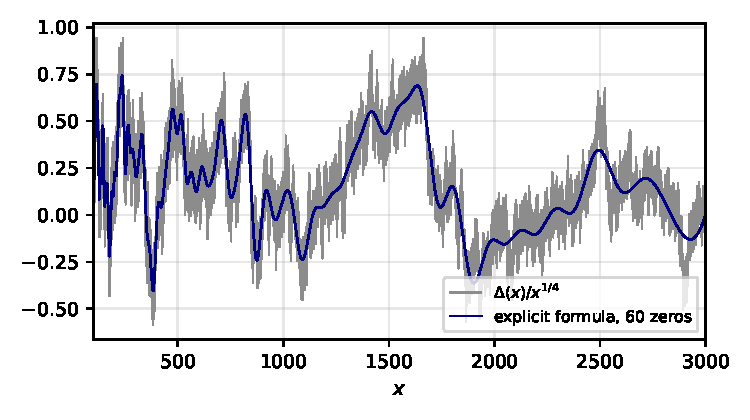
\includegraphics[width=0.8\textwidth]{fig/sqfree_atoms.pdf}
\caption{The normalised error $\Delta(x)/x^{1/4}$ of the squarefree count on $[100,3000]$ (grey) and the explicit formula \eqref{eq:sqfree:explicit} with the first $60$ zeros and the trivial terms at $s=-1$, $-3$ and $-5$, divided by $x^{1/4}$ (dark). Drawn by \texttt{sqfree\_atoms.py}.}
\label{fig:sqfree:atoms}
\end{figure}

For the sum $\sum_{n\le x}\mu(n)^2/n$ of Proposition~\ref{prop:sqfree:alpha1} the same atoms appear at $s=\rho/2-1$, with residues $\zeta(\rho/2)x^{\rho/2-1}/((\rho-2)\zeta'(\rho))$ of size $x^{-3/4}$ under RH (of modulus $0.09991\,x^{-3/4}$ for the first zero), inside the error $O(x^{-1/2})$. Likewise the error $\mathcal E_\alpha$ of \eqref{eq:sqfree:alpha}, for $\frac12<\alpha<1$, has atoms of size $x^{1/4-\alpha}$. By \eqref{eq:sqfree:Ealpha}, a pointwise bound of that order in either case would follow from $\Delta(x)=O(x^{1/4+\varepsilon})$, and it is open for the same reason.

\subsection{Smoothed counts}\label{sec:sqfree:smooth}

Smoothing the count removes the obstacle. For $x>0$ let
\[
Q_1(x)=\sum_{n\ge1}\mu(n)^2e^{-n/x}=\sum_{d\ge1}\frac{\mu(d)}{e^{d^2/x}-1},\qquad Q_2(x)=\sum_{n\ge1}\mu(n)^2\Big(1+\frac{2n}x\Big)e^{-2n/x},
\]
the second form of $Q_1$ by $\mu(n)^2=\sum_{d^2\mid n}\mu(d)$. If $G_{1,x}$ is exponential and $G_{2,x}$ has the Gamma(2) law, both with mean $x$, then $P(G_{1,x}\ge n)=e^{-n/x}$ and $P(G_{2,x}\ge n)=(1+2n/x)e^{-2n/x}$, so $Q_1(x)=\E Q(G_{1,x})$ and $Q_2(x)=\E Q(G_{2,x})$. Since $\int_0^\infty e^{-n/x}x^{-s-1}dx=\Gamma(s)n^{-s}$ and $\int_0^\infty(1+2n/x)e^{-2n/x}x^{-s-1}dx=(1+s)\Gamma(s)(2n)^{-s}$, the Mellin transforms are
\begin{equation}\label{eq:sqfree:mellin12}
\begin{aligned}
\int_0^\infty Q_1(x)\,x^{-s-1}dx&=\Gamma(s)D(s),\\
\int_0^\infty Q_2(x)\,x^{-s-1}dx&=(1+s)\Gamma(s)\,2^{-s}D(s),\qquad\re s>1 .
\end{aligned}
\end{equation}
The kernels $\Gamma(s)$ and $(1+s)\Gamma(s)2^{-s}$ have no zeros in $\re s>0$ and decay exponentially on vertical lines.

\begin{lemma}\label{lem:sqfree:descent}
If $D(s)=\zeta(s)/\zeta(2s)$ is analytic in the half plane $\re s>\frac14$ apart from $s=1$, then RH holds.
\end{lemma}

\begin{proof}
Let $\rho$ be a zero with $\beta=\re\rho>\frac12$. Then $\re(\rho/2)>\frac14$, so the pole of $1/\zeta(2s)$ at $s=\rho/2$ must be cancelled, that is $\zeta(\rho/2)=0$. Since $\frac14<\re(\rho/2)<\frac12$, the functional equation and the reflection $s\mapsto\bar s$ make $\rho'=1-\bar\rho/2$ a zero, with $\re\rho'=1-\beta/2>\frac12$ and $\im\rho'=\im\rho/2$. Iterating gives zeros $\rho_j$ whose real parts tend to $\frac23$, the fixed point of $\beta\mapsto1-\beta/2$, and whose imaginary parts are $\im\rho/2^j$. Since $\zeta<0$ on $(0,1)$, $\im\rho\ne0$, so the $\rho_j$ are distinct and accumulate at $\frac23$, where $\zeta$ is analytic and not identically zero, a contradiction.
\end{proof}

\begin{theorem}\label{thm:sqfree:smooth}
\textup{(i)} RH holds if and only if $Q_1(x)=\frac6{\pi^2}x+O(x^{1/4+\varepsilon})$ for every $\varepsilon>0$, and if and only if $Q_2(x)=\frac6{\pi^2}x+O(x^{1/4+\varepsilon})$ for every $\varepsilon>0$.

\textup{(ii)} Under RH, if the zeros are simple, then
\begin{align*}
Q_1(x)&=\frac6{\pi^2}x+1+\sum_\rho A_\rho\,x^{\rho/2}+\frac{c_1\log x+c_2}x+O(x^{-2}),\\
Q_2(x)&=\frac6{\pi^2}x+1+\sum_\rho B_\rho\,x^{\rho/2}+\frac{2c_1}x+O(x^{-2}),\\
A_\rho&=\frac{\Gamma(\rho/2)\,\zeta(\rho/2)}{2\zeta'(\rho)},\qquad B_\rho=\Big(1+\frac\rho2\Big)\frac{2^{-\rho/2}\,\Gamma(\rho/2)\,\zeta(\rho/2)}{2\zeta'(\rho)},
\end{align*}
the sums over $\rho$ taken over $|\im\rho|<2T_j$ along a sequence $T_j\to\infty$, with
\begin{align*}
c_1&=-\frac{\zeta(-1)}{2\zeta'(-2)}=-1.36843277762021,\\
c_2&=c_1\Big(1-\gamma_E+\frac{\zeta'(-1)}{\zeta(-1)}-\frac{\zeta''(-2)}{\zeta'(-2)}\Big)=-0.339381226129599 .
\end{align*}
\end{theorem}

\begin{proof}
(i) Suppose RH. By Section~14.2 of \cite{Titchmarsh}, $1/\zeta(\sigma+it)=O(|t|^\varepsilon)$ uniformly for $\sigma\ge\frac12+\varepsilon$, and $\zeta(\sigma+it)$ grows at most polynomially in $|t|$ on vertical strips, while $\Gamma(s)$ decays exponentially. Move the line of integration in $Q_1(x)=\frac1{2\pi i}\int_{(2)}\Gamma(s)D(s)x^s\,ds$ to $\re s=\frac14+\varepsilon$. The only pole crossed is $s=1$, with residue $\Gamma(1)/\zeta(2)\cdot x=6x/\pi^2$; the point $s=\frac12$ is regular because $\zeta(2s)$ has a pole there. On the new line $|\Gamma(s)D(s)|$ is integrable and the integral is $O(x^{1/4+\varepsilon})$. The same argument with the kernel $(1+s)\Gamma(s)2^{-s}$ treats $Q_2$.

Conversely, suppose $Q_1(x)=\frac6{\pi^2}x+O(x^{1/4+\varepsilon})$ for every $\varepsilon>0$. For $\re s>1$, by \eqref{eq:sqfree:mellin12},
\[
\Gamma(s)D(s)-\frac6{\pi^2}\,\frac1{s-1}=\int_1^\infty\Big(Q_1(x)-\frac6{\pi^2}x\Big)x^{-s-1}dx+\int_0^1Q_1(x)\,x^{-s-1}dx .
\]
The first integral converges and is analytic in $\re s>\frac14$, by the hypothesis, and the second is entire, since $Q_1(x)=O(e^{-1/x})$ as $x\to0$. As $\Gamma$ has no zeros, $D$ is analytic in $\re s>\frac14$ apart from $s=1$, and Lemma~\ref{lem:sqfree:descent} gives RH. The same argument applies to $Q_2$.

(ii) By Theorem~9.7 of \cite{Titchmarsh} there are heights $T_j\in[j,j+1]$ at which $1/\zeta(\sigma\pm2iT_j)=T_j^{O(1)}$ uniformly for $-1\le\sigma\le2$, and on the left of the line $\re s=-\frac12$ the functional equation bounds $1/\zeta(2s)$ polynomially. Move the line of integration to $\re s=-\frac52$ along the rectangles of height $T_j$; the exponential decay of $\Gamma$ makes the horizontal sides vanish as $j\to\infty$, and the integral on the new line is $O(x^{-5/2})$. The poles crossed are $s=1$; the points $\rho/2$, with the residues $A_\rho x^{\rho/2}$ and $B_\rho x^{\rho/2}$; $s=0$, where $\Gamma(s)D(s)$ and $(1+s)\Gamma(s)2^{-s}D(s)$ have residue $D(0)=\zeta(0)/\zeta(0)=1$; $s=-1$; and $s=-2$, a simple pole of both, which gives a multiple of $x^{-2}$. At $s=-1$, $\Gamma$ has a simple pole and $1/\zeta(2s)$ another, from the trivial zero $-2$ of $\zeta$, so $\Gamma(s)D(s)=c_1(s+1)^{-2}+c_2(s+1)^{-1}+O(1)$, with $c_1$ and $c_2$ from the expansions $\Gamma(s)=-(s+1)^{-1}(1+(1-\gamma_E)(s+1)+\cdots)$, $\zeta(s)=\zeta(-1)(1+\frac{\zeta'(-1)}{\zeta(-1)}(s+1)+\cdots)$ and $\zeta(2s)=2\zeta'(-2)(s+1)(1+\frac{\zeta''(-2)}{\zeta'(-2)}(s+1)+\cdots)$, and the residue of $\Gamma(s)D(s)x^s$ is $x^{-1}(c_1\log x+c_2)$. The factor $1+s$ makes the pole of $(1+s)\Gamma(s)2^{-s}D(s)$ at $s=-1$ simple, with residue $2c_1$ times $x^{-1}$.
\end{proof}

At the even negative integers $\Gamma(s)D(s)$ has simple poles, since $\zeta(s)$ vanishes there together with $\zeta(2s)$, and at the odd ones double poles: \texttt{sqfree\_smooth.py} computes the Laurent coefficients at $s=-1,\dots,-6$ by the trapezoid rule on circles of radius $0.3$ and reproduces the closed forms of $c_1$ and $c_2$ within $5\times10^{-46}$. For $Q_2$ the double pole at $s=-1$ becomes a simple one, with residue $2c_1$.

The coefficients $A_\rho$ are tiny, $|A_{\rho_1}|=1.648\times10^{-5}$ and $6.29\times10^{-82}$ at the hundredth zero, because $|\Gamma(\rho/2)|$ decays like $e^{-\pi\gamma/4}$. \texttt{sqfree\_smooth.py} checks part~(ii) for $Q_1$: the smoothed error is the sum of the atom terms and the trivial terms to the working precision. Table~\ref{tab:sqfree:gamma2} in Section~\ref{sec:sqfree:mertens} does the same for $Q_2$.

The Perron kernel $x^s/s$ decays only like $1/|t|$, so the atom series for $Q(x)$ has no exponential damping, and bounding its partial sums would need control of $\sum_{|\gamma|\le T}|\zeta(\rho/2)/(\rho\zeta'(\rho))|$, which is out of reach.

\subsection{Mean square, and how much smoothing the sharp count needs}\label{sec:sqfree:meansq}

Two further results bracket the sharp problem. The first settles it on average; it is presumably folklore. For $\re s>1$ let
\[
F(s)=\int_1^\infty\Delta(x)\,x^{-s-1}dx=\frac{D(s)}s-\frac6{\pi^2}\,\frac1{s-1},
\]
the second form because $\int_1^\infty Q(x)x^{-s-1}dx=D(s)/s$.

\begin{theorem}\label{thm:sqfree:meansq}
RH holds if and only if $\int_X^{2X}\Delta(x)^2\,dx=O(X^{3/2+\varepsilon})$ for every $\varepsilon>0$, that is, if and only if the root mean square of $\Delta$ on every range $[X,2X]$ is $O(X^{1/4+\varepsilon})$.
\end{theorem}

\begin{proof}
Suppose RH. Then $F$ continues analytically to $\re s>\frac14$: the poles of $D$ at the points $\rho/2$ lie on the line $\re s=\frac14$, $s=\frac12$ is regular, and the pole at $s=1$ cancels. By Section~14.2 of \cite{Titchmarsh}, under RH $\zeta(\sigma+it)=O(|t|^{\max(0,\frac12-\sigma)+\varepsilon})$ and $1/\zeta(2\sigma+2it)=O(|t|^\varepsilon)$ uniformly for $\sigma\ge\frac14+\varepsilon$ and $|t|\ge1$, so $F(\sigma+it)=O(|t|^{-3/4+2\varepsilon})$ uniformly there. For $w>2$ let $I(w)=\int_1^\infty\Delta(x)^2x^{-w-1}dx$, the Laplace transform in $v=\log x$ of the nonnegative function $\Delta(e^v)^2$. Plancherel's theorem for the function $v\mapsto\Delta(e^v)e^{-wv/2}$ on $(0,\infty)$, whose Fourier transform is $t\mapsto F(\frac w2+it)$, and the symmetry $F(\bar s)=\overline{F(s)}$ give
\[
I(w)=\frac1{2\pi}\int_{-\infty}^\infty F\Big(\frac w2+it\Big)\,F\Big(\frac w2-it\Big)\,dt,\qquad w>2 .
\]
The right side is analytic in $w$ on $\re w>\frac12$, since the integrand is analytic there and $O(|t|^{-3/2+4\varepsilon})$ locally uniformly. So $I$, the Laplace transform of a nonnegative function, continues analytically to a neighbourhood of every point of $(\frac12,\infty)$, and Landau's theorem \cite[Chapter~II, Theorem~5b]{Widder41} puts its abscissa of convergence at or below $\frac12$. Hence $I(w)<\infty$ for every $w>\frac12$, and $\int_X^{2X}\Delta^2\,dx\le(2X)^{w+1}I(w)=O(X^{3/2+\varepsilon})$ with $w=\frac12+\varepsilon$.

Conversely, by the Cauchy Schwarz inequality the hypothesis gives $\int_X^{2X}|\Delta(x)|x^{-\sigma-1}dx=O(X^{1/4+\varepsilon-\sigma})$, so, summing over $X=2^j$, the integral defining $F$ converges absolutely for $\re s>\frac14$. Then $D(s)=s\big(F(s)+\frac6{\pi^2}\frac1{s-1}\big)$ is analytic in $\re s>\frac14$ apart from $s=1$, and Lemma~\ref{lem:sqfree:descent} gives RH.
\end{proof}

Table~\ref{tab:sqfree:rms} gives the root mean square of $\Delta$ on dyadic ranges, computed exactly from the sieve: on $[n,n+1)$ the error decreases linearly from $\Delta_n=Q(n)-6n/\pi^2$ to $\Delta_n-6/\pi^2$, so $\int_n^{n+1}\Delta^2=\Delta_n^2-\frac6{\pi^2}\Delta_n+\frac{12}{\pi^4}$, and the extremes over real $x$ are taken at integers or as left limits there. Over the eighteen ranges $[X,2X]$ with $X=10^4\cdot2^j$, $j=0,\dots,13$, and $X=10^4,\dots,10^8$, the root mean square divided by $X^{1/4}$ lies between $0.2337$ and $0.3606$ and the largest $|\Delta(x)|/X^{1/4}$ between $0.6851$ and $1.0361$; on $[10^3,2\times10^8]$ the largest value of $\Delta(x)/x^{1/4}$ is $0.9807$, near $x=47523$, and the least $-0.8685$, near $x=80157$.

\begin{table}[htbp]
\centering\small
\begin{tabular}{rccc}
\toprule
$X$ & $\big(\frac1X\int_X^{2X}\Delta^2\big)^{1/2}\big/X^{1/4}$ & $\max_{[X,2X]}|\Delta(x)|/X^{1/4}$ & near $x=$\\
\midrule
$10^4$ & $0.2701$ & $0.8979$ & $18471$\\
$10^5$ & $0.2494$ & $0.6851$ & $128599$\\
$10^6$ & $0.2779$ & $0.8382$ & $1618611$\\
$10^7$ & $0.3541$ & $0.9931$ & $17199381$\\
$10^8$ & $0.2812$ & $0.8636$ & $144151023$\\
\bottomrule
\end{tabular}
\caption{Root mean square and largest absolute value of the squarefree error $\Delta$ on the ranges $[X,2X]$, divided by $X^{1/4}$, over real $x$; the largest value on $[10^7,2\times10^7]$ is the left limit at $17199381$, and over the integers alone it is $0.982$. Computed by \texttt{sqfree\_sieve.py}.}
\label{tab:sqfree:rms}
\end{table}

\begin{corollary}\label{cor:sqfree:omega}
\textup{(i)} Under RH, for every $\varepsilon>0$ the set of $x\in[X,2X]$ with $|\Delta(x)|>X^{1/4+\varepsilon}$ has measure $O(X^{1-\varepsilon})$.

\textup{(ii)} With no hypothesis,
\[
\limsup_{x\to\infty}\frac{\Delta(x)}{x^{1/4}}\ge|R_{\rho_1}|,\qquad\liminf_{x\to\infty}\frac{\Delta(x)}{x^{1/4}}\le-|R_{\rho_1}|,
\]
where $R_{\rho_1}=\zeta(\rho_1/2)/(\rho_1\zeta'(\rho_1))$ and $|R_{\rho_1}|=0.100404$. The same holds for $Q_2(x)-\frac6{\pi^2}x-1$ with $|B_{\rho_1}|=9.944\times10^{-5}$ in place of $|R_{\rho_1}|$.
\end{corollary}

\begin{proof}
(i) is Chebyshev's inequality applied to Theorem~\ref{thm:sqfree:meansq}. For (ii) suppose that $\Delta(x)\le c\,x^{1/4}$ for $x\ge x_0$, with $0<c<|R_{\rho_1}|$. The function $L(s)=\int_{x_0}^\infty(cx^{1/4}-\Delta(x))x^{-s-1}dx$ is the Laplace transform in $\log x$ of a nonnegative function, and for $\re s>1$
\[
L(s)=\frac{c\,x_0^{1/4-s}}{s-\frac14}-F(s)+E(s),
\]
with $E$ entire. The right side has no singularity on the real half line $(\frac14,\infty)$: a real pole of $D$ there would be a real zero of $\zeta$ in $(\frac12,\infty)$, of which there are none, $s=\frac12$ is regular, and the pole at $s=1$ cancels. By Landau's theorem the integral $L(s)$ converges for $\re s>\frac14$, so $F$ is analytic there (which already gives RH, by Lemma~\ref{lem:sqfree:descent}), and $|L(\sigma+it)|\le L(\sigma)$ for $\sigma>\frac14$. As $\sigma\downarrow\frac14$, $L(\sigma)=c/(\sigma-\frac14)+O(1)$, since $F$ is analytic at $s=\frac14$, where $\zeta(2s)=\zeta(\frac12)\ne0$. At $s=\sigma+\frac i2\gamma_1$ the first and last terms of the display are $O(1)$, while $F(s)=R_{\rho_1}/(\sigma-\frac14)+O(1)$, because $D(s)/s$ has a simple pole at $\rho_1/2$ with residue $R_{\rho_1}$ (the zero $\rho_1$ is simple and $\zeta(\rho_1/2)\ne0$). Hence $|R_{\rho_1}|\le c$, a contradiction. The lower bound is the same argument applied to $c\,x^{1/4}+\Delta(x)$, and the smoothed case is the same argument with the kernel $(1+s)\Gamma(s)2^{-s}$, whose residue at $\rho_1/2$ is $B_{\rho_1}$.
\end{proof}



The second result measures the cost of sharpening. Let $G_{n,x}$ have the Gamma($n$) law with mean $x$, so that $G_{n,x}$ concentrates at $x$ in a window of width $x/\sqrt n$; $Q_1(x)=\E Q(G_{1,x})$ and $Q_2(x)=\E Q(G_{2,x})$.

\begin{proposition}\label{prop:sqfree:gamman}
Under RH, uniformly in $n\ge1$,
\[
\E Q(G_{n,x})=\frac6{\pi^2}\,x+O_\varepsilon\big(x^{1/4+\varepsilon}\,n^{1/8+\varepsilon}\big).
\]
\end{proposition}

\begin{proof}
With rate $\lambda=n/x$, $P(G_{n,x}\ge m)=\Gamma(n,\lambda m)/\Gamma(n)$, whose Mellin transform in $\lambda m$ is $\Gamma(s+n)/(s\Gamma(n))$, so $\E Q(G_{n,x})=\frac1{2\pi i}\int_{(2)}D(s)\frac{\Gamma(s+n)}{s\Gamma(n)}\big(\frac xn\big)^sds$. Move the line to $\re s=c=\frac14+\varepsilon$, collecting $6x/\pi^2$ at $s=1$. On the new line $|\Gamma(n+c+it)|/\Gamma(n)=O\big(n^c\exp(-\kappa\min(t^2/n,|t|))\big)$ for an absolute $\kappa>0$, since $\Gamma(n+c)/\Gamma(n)=O(n^c)$ and $|\Gamma(n+c+it)/\Gamma(n+c)|^2=\prod_{k\ge0}\big(1+t^2/(n+c+k)^2\big)^{-1}$; the factors with $k<n$ give $e^{-\kappa t^2/n}$ when $|t|\le n$, and those with $k\le|t|$ give $e^{-\kappa|t|}$ when $|t|>n$. Under RH, $|D(c+it)|=O(|t|^{1/4+\varepsilon})$ for $|t|\ge1$ (Section~14.2 of \cite{Titchmarsh} and the functional equation). The remaining integral is therefore $O\big(x^c\int(1+|t|)^{-3/4+\varepsilon}e^{-\kappa\min(t^2/n,|t|)}dt\big)=O(x^cn^{1/8+\varepsilon})$, the integral being dominated by $|t|\lesssim\sqrt n$.
\end{proof}

Balancing the window against the loss gives a bound for the sharp count.

\begin{corollary}\label{cor:sqfree:twofifths}
Under RH, $\Delta(x)=O(x^{2/5+\varepsilon})$ for every $\varepsilon>0$.
\end{corollary}

\begin{proof}
Since $Q$ is nondecreasing and counts integers, $|Q(y)-Q(x)|\le|y-x|+1$, so $|\E Q(G_{n,x})-Q(x)|\le\E|G_{n,x}-x|+1\le x/\sqrt n+1$. With Proposition~\ref{prop:sqfree:gamman}, $\Delta(x)=O(x^{1/4+\varepsilon}n^{1/8+\varepsilon}+x/\sqrt n)$, and $n=\lceil x^{6/5}\rceil$ balances the two terms at $x^{2/5+O(\varepsilon)}$.
\end{proof}

The exponent $\frac25$ is weaker than the known conditional exponents. If the loss $n^{1/8}$ were replaced by $n^\delta$, the same balance would give $\Delta(x)=O(x^{1-3/(8\delta+4)+\varepsilon})$, which tends to $x^{1/4+\varepsilon}$ as $\delta\to0$; conversely $\Delta(x)=O(x^{1/4+\varepsilon})$ gives $|\E Q(G_{n,x})-\frac6{\pi^2}x|\le\E|\Delta(G_{n,x})|=O(x^{1/4+\varepsilon})$ uniformly in $n$, by Jensen's inequality. So the sharp conjecture amounts to removing the loss, which needs cancellation in $\int_{|t|\le T}D(\frac14+it)x^{it}\,dt/t$ and not only a bound on the size of the integrand.

\subsection{Gamma(2) smoothing and the Mertens function}\label{sec:sqfree:mertens}

The elementary method rests on the terms $\mu(d)(\lfloor x/d^2\rfloor-x/d^2)=-\mu(d)\{x/d^2\}$ of \eqref{eq:sqfree:Qd}. Following the idea of Steutel and Thiemann of splitting a random variable into its integer and fractional parts \cite{SteutelThiemann89}, we randomise $x$ by a gamma law. Theorem~\ref{thm:sqfree:threshold} shows that here shape two is the largest for which the average is taken under a positive law.

Let $Y$ have the Gamma($\nu$) law with rate $\lambda$, let $a>0$ and $y=\lambda a$. Then $\E\lfloor Y/a\rfloor=\sum_{m\ge1}P(Y\ge ma)=\sum_{m\ge1}\Gamma(\nu,my)/\Gamma(\nu)$ and $\E Y/a=\nu/y$, so the expected fractional part is
\[
\E\{Y/a\}=g_\nu(y)=\frac\nu y-\sum_{m\ge1}\frac{\Gamma(\nu,my)}{\Gamma(\nu)} .
\]
For $\nu=1$, Steutel and Thiemann observed that $\lfloor Y/a\rfloor$ is geometric and $\{Y/a\}$ an independent truncated exponential variable, with $\E\lfloor Y/a\rfloor=1/(e^y-1)$ and $g_1(y)=1/y-1/(e^y-1)$.

\begin{lemma}\label{lem:sqfree:frac2}
For $\nu=2$,
\[
\E\lfloor Y/a\rfloor=\frac1{e^y-1}+\frac y{4\sinh^2(y/2)},\qquad g_2(y)=\frac2y-\frac1{e^y-1}-\frac y{4\sinh^2(y/2)} .
\]
For $0<|y|<2\pi$, with the Bernoulli numbers $B_{2k}$,
\[
g_2(y)=\frac12+\sum_{k\ge2}\frac{(2k-2)B_{2k}}{(2k)!}\,y^{2k-1}=\frac12-\frac{y^3}{360}+\frac{y^5}{7560}-\cdots,
\]
$g_2(y)=2/y+O(ye^{-y})$ as $y\to\infty$, and for every $\nu>0$
\[
\int_0^\infty g_\nu(y)\,y^{s-1}\,dy=-\frac{\Gamma(s+\nu)\,\zeta(s)}{s\,\Gamma(\nu)},\qquad 0<\re s<1,
\]
which is $-(1+s)\Gamma(s)\zeta(s)$ for $\nu=2$.
\end{lemma}

\begin{proof}
For $\nu=2$, $P(Y\ge ma)=(1+my)e^{-my}$, and $\sum_me^{-my}=1/(e^y-1)$, $\sum_mmye^{-my}=y/(4\sinh^2(y/2))$. For the expansion use $1/(e^y-1)=1/y-\frac12+\sum_{k\ge1}B_{2k}y^{2k-1}/(2k)!$ and $y/(4\sinh^2(y/2))=-y\frac d{dy}(e^y-1)^{-1}$. For the Mellin transform write $g_\nu(y)=\E\{Y/y\}$ with $Y$ of law Gamma($\nu$,1), substitute $u=Y/y$, and use the classical formula $\int_0^\infty\{u\}u^{-s-1}du=-\zeta(s)/s$ for $0<\re s<1$ \cite[Section~2.1]{Titchmarsh}: the transform is $\E Y^s\cdot(-\zeta(s)/s)$, with $\E Y^s=\Gamma(s+\nu)/\Gamma(\nu)$.
\end{proof}

The terms of the elementary method now read $\E\big[\mu(d)\big(\lfloor G_{2,x}/d^2\rfloor-G_{2,x}/d^2\big)\big]=-\mu(d)g_2(2d^2/x)$ for $G_{2,x}$ of the Gamma(2) law with mean $x$, and since $0\le g_2(y)\le\min(1,2/y)$ the sum over all $d$ converges absolutely, with no truncation at $d^2\le x$:
\begin{equation}\label{eq:sqfree:EQ}
Q_2(x)=\sum_{n\ge1}\mu(n)^2\Big(1+\frac{2n}x\Big)e^{-2n/x}=\frac6{\pi^2}\,x-\sum_{d\ge1}\mu(d)\,g_2\Big(\frac{2d^2}x\Big).
\end{equation}

\begin{theorem}\label{thm:sqfree:mertens}
Let
\[
f_2(y)=-2g_2'(y)=\frac4{y^2}-\frac{y\cosh(y/2)}{2\sinh^3(y/2)},\qquad y>0 .
\]
Then $f_2>0$, $f_2(y)=y^2/60+O(y^4)$ as $y\to0$ and $f_2(y)\sim4/y^2$ as $y\to\infty$, and $f_2$ is the density of a probability law $\mathcal V_2$ with $P(\mathcal V_2\ge y)=2g_2(y)$ and
\[
\E\mathcal V_2^s=-2\,\Gamma(s+2)\,\zeta(s),\qquad -3<\re s<1 .
\]
For every $x>0$,
\[
Q_2(x)=\frac6{\pi^2}\,x-\frac12\,\E M\Big(\sqrt{x\mathcal V_2/2}\Big).
\]
Moreover $f_2$ is twice the difference between the continuous and the integer mixtures of the Gamma(2) densities $\gamma_{2,\lambda}(y)=\lambda^2ye^{-\lambda y}$ over their rate:
\[
f_2(y)=2\Big(\int_0^\infty\gamma_{2,\lambda}(y)\,d\lambda-\sum_{m\ge1}\gamma_{2,m}(y)\Big)=-2\int_0^\infty\Big(\{\lambda\}-\frac12\Big)\,\partial_\lambda\gamma_{2,\lambda}(y)\,d\lambda .
\]
\end{theorem}

\begin{proof}
With $z=y/2$, $f_2(y)>0$ is $(\sinh z/z)^3>\cosh z$, Lazarevi\'c's inequality \cite{Lazarevic66}. The expansion at $0$ follows from Lemma~\ref{lem:sqfree:frac2}. The mass is $2(g_2(0+)-g_2(\infty))=1$ and the tail is $2g_2(y)$. Integrating by parts in the Mellin formula of Lemma~\ref{lem:sqfree:frac2} gives $\E\mathcal V_2^s=2s\int_0^\infty y^{s-1}g_2(y)\,dy=-2s(1+s)\Gamma(s)\zeta(s)$ for $0<\re s<1$, and the behaviour at $0$ and at infinity extends the integral and the identity to $-3<\re s<1$. For the representation, $P(\sqrt{x\mathcal V_2/2}\ge d)=P(\mathcal V_2\ge2d^2/x)=2g_2(2d^2/x)$, so $\frac12\E M(\sqrt{x\mathcal V_2/2})=\sum_d\mu(d)g_2(2d^2/x)$, the interchange being justified by absolute convergence, and \eqref{eq:sqfree:EQ} gives the formula. Finally $\int_0^\infty\gamma_{2,\lambda}(y)\,d\lambda=2/y^2$ and $\sum_m\gamma_{2,m}(y)=y\sum_mm^2e^{-my}=y\cosh(y/2)/(4\sinh^3(y/2))$, and the last form is the Euler Maclaurin formula $\int_0^\infty h-\sum_{m\ge1}h(m)=-\int_0^\infty(\{\lambda\}-\frac12)h'(\lambda)\,d\lambda$ for $h=\gamma_{2,\cdot}(y)$, which vanishes at $\lambda=0$.
\end{proof}

The exponential case is the same with
\[
f_1(y)=-2g_1'(y)=\frac2{y^2}-\frac1{2\sinh^2(y/2)}=2\Big(\int_0^\infty\lambda e^{-\lambda y}d\lambda-\sum_{m\ge1}me^{-my}\Big)>0,
\]
positive because $\sinh z>z$, with $f_1(0+)=\frac16$, $\E\mathcal V_1^s=-2\Gamma(s+1)\zeta(s)$ for $-1<\re s<1$, and
\[
Q_1(x)=\frac6{\pi^2}\,x-\frac12\,\E M\Big(\sqrt{x\mathcal V_1}\Big).
\]

\begin{corollary}\label{cor:sqfree:mertens}
\textup{(i)} With no hypothesis, $Q_\nu(x)=\frac6{\pi^2}x+o(x^{1/2})$ for $\nu=1,2$. \textup{(ii)} Under RH, $|Q_2(x)-\frac6{\pi^2}x|\le\frac12\E|M(\sqrt{x\mathcal V_2/2})|=O(x^{1/4+\varepsilon})$, and likewise for $Q_1$; this is a second proof of the forward half of Theorem~\ref{thm:sqfree:smooth}(i).
\end{corollary}

\begin{proof}
(i) $|M(t)|\le t$ and $M(t)=o(t)$, and $\E\mathcal V_\nu^{1/2}<\infty$, so dominated convergence gives $\E M(\sqrt{x\mathcal V_2/2})=o(x^{1/2})$, and likewise for $\mathcal V_1$. (ii) RH gives $M(t)=O(t^{1/2+\varepsilon})$ \cite[Section~14.25]{Titchmarsh}, and $\E\mathcal V_\nu^{1/4+\varepsilon}<\infty$.
\end{proof}

Table~\ref{tab:sqfree:gamma2} checks \eqref{eq:sqfree:EQ} and Theorem~\ref{thm:sqfree:smooth}(ii) for $Q_2$. It computes $Q_2(x)=\sum_d\mu(d)\,\E\lfloor G_{2,x}/d^2\rfloor=\sum_d\mu(d)\big(1/(e^t-1)+t/(4\sinh^2(t/2))\big)$, $t=2d^2/x$, whose terms with $t>140$ are below $10^{-55}$, and this agrees with the direct sum over $n$, in double precision, within $10^{-10}$ up to $x=10^6$. The sum \eqref{eq:sqfree:EQ} truncated at $d\le2\times10^5$, as in the first author's note, loses $2.2\times10^{-4}$ at $x=10^6$, because $g_2(2d^2/x)$ is close to $x/d^2$ for large $d$ and the tail $x\sum_{d>2\times10^5}\mu(d)/d^2$ is left out.

\begin{table}[htbp]
\centering\footnotesize
\setlength{\tabcolsep}{3.5pt}
\fitwidth{\begin{tabular}{rcccccc}
\toprule
$x$ & $Q_2(x)-\frac6{\pi^2}x$ & $d\le2\cdot10^5$ & $\frac{Q_2(x)-\frac6{\pi^2}x-1}{x^{1/4}}$ & $100$ atoms & trivial terms & residual\\
\midrule
$10^3$ & $0.997161220898$ & $0.997161002208$ & $-5.048\times10^{-4}$ & $-1.0571\times10^{-4}$ & $-2.73307\times10^{-3}$ & $-1.0\times10^{-23}$\\
$10^4$ & $1.00094524529$ & $1.00094305839$ & $9.452\times10^{-5}$ & $1.21889\times10^{-3}$ & $-2.73648\times10^{-4}$ & $-1.3\times10^{-30}$\\
$10^5$ & $0.996620193442$ & $0.99659832449$ & $-1.9006\times10^{-4}$ & $-3.35244\times10^{-3}$ & $-2.73683\times10^{-5}$ & $-1.5\times10^{-37}$\\
$10^6$ & $1.00610290943$ & $1.00588421991$ & $1.9299\times10^{-4}$ & $6.10565\times10^{-3}$ & $-2.73686\times10^{-6}$ & $-1.8\times10^{-41}$\\
$10^7$ & $0.992114718377$ & & $-1.4022\times10^{-4}$ & $-7.88501\times10^{-3}$ & $-2.73687\times10^{-7}$ & $-3.9\times10^{-42}$\\
$10^8$ & $1.00440085379$ & & $4.4009\times10^{-5}$ & $4.40088\times10^{-3}$ & $-2.73687\times10^{-8}$ & $-2.2\times10^{-38}$\\
\bottomrule
\end{tabular}}
\caption{The Gamma(2) smoothed count: $Q_2(x)-6x/\pi^2$, the sum \eqref{eq:sqfree:EQ} truncated at $d\le2\times10^5$, the normalised error, the contribution $2\re\sum_{k\le100}B_{\rho_k}x^{\rho_k/2}$ of the first hundred atoms, the residues at $s=-1,\dots,-6$, whose leading part is $2c_1/x$, and the residual. The constant $1$ is the residue $D(0)$ at $s=0$. Computed by \texttt{sqfree\_smooth.py} at $45$ digits.}
\label{tab:sqfree:gamma2}
\end{table}

\subsection{Gamma shapes: two is the threshold}\label{sec:sqfree:shape}

For every real shape $\nu>0$, $f_\nu=-2g_\nu'$ is a signed density of total mass $2g_\nu(0+)=1$, and the argument of Theorem~\ref{thm:sqfree:mertens} gives, for $Y$ of the Gamma($\nu$) law with rate $\lambda$,
\begin{gather*}
\E Q(Y)=\frac6{\pi^2}\,\E Y-\frac12\int_0^\infty M\Big(\sqrt{y/\lambda}\Big)f_\nu(y)\,dy,\\
\int_0^\infty y^sf_\nu(y)\,dy=-\frac{2\,\Gamma(s+\nu)\,\zeta(s)}{\Gamma(\nu)},\qquad -\nu<\re s<1 .
\end{gather*}


Write $\gamma_a(t)=t^{a-1}e^{-t}/\Gamma(a)$ for the Gamma($a$) density, and let
\begin{gather*}
\mathcal R_\nu(y)=y\sum_{m\ge1}\gamma_{\nu+1}(my)=\frac{y^{\nu+1}}{\Gamma(\nu+1)}\sum_{m\ge1}m^\nu e^{-my},\\
q_\nu(y)=\frac{\Gamma(\nu+1)\,\big(1-\mathcal R_\nu(y)\big)}{y^{\nu+1}},
\end{gather*}
so that $\mathcal R_\nu(y)$ is the right Riemann sum with step $y$ of the Gamma($\nu+1$) density, whose integral is $1$.

\begin{lemma}\label{lem:sqfree:riemann}
For $\nu>0$ and $y>0$,
\[
f_\nu(y)=\frac{2\nu\big(1-\mathcal R_\nu(y)\big)}{y^2}=\frac{2y^{\nu-1}}{\Gamma(\nu)}\,q_\nu(y),
\]
so $f_\nu\ge0$ exactly when $\mathcal R_\nu\le1$. For $0<y<2\pi$,
\[
q_\nu(y)=-\sum_{k\ge0}\zeta(-\nu-k)\,\frac{(-y)^k}{k!},
\]
and $\mathcal R_1(y)=(y/2)^2/\sinh^2(y/2)$, $\mathcal R_2(y)=(y/2)^3\cosh(y/2)/\sinh^3(y/2)$.
\end{lemma}

\begin{proof}
With $Y$ of the Gamma($\nu$,1) law and $c=1/y$, $g_\nu(y)=\E\{cY\}=c\nu-\sum_{m\ge1}P(Y\ge m/c)$, whose derivative in $c$ is $\nu-\sum_m(m/c^2)p_\nu(m/c)$, with $p_\nu=\gamma_\nu$ the density of $Y$. Since $tp_\nu(t)=\nu\gamma_{\nu+1}(t)$, the derivative is $\nu(1-\mathcal R_\nu(1/c))$, and returning to $y$ gives $g_\nu'(y)=-\nu(1-\mathcal R_\nu(y))/y^2$. The series is the expansion $\sum_mm^\nu e^{-my}=\Gamma(\nu+1)y^{-\nu-1}+\sum_{k\ge0}\zeta(-\nu-k)(-y)^k/k!$ of the polylogarithm, valid for $0<y<2\pi$.
\end{proof}

So $\mathcal R_1\le1$ is $\sinh z\ge z$ and $\mathcal R_2\le1$ is Lazarevi\'c's inequality. Near the origin $f_\nu$ has the sign of $q_\nu(0+)=-\zeta(-\nu)$, and at an even integer $\nu=2m$, where $\zeta(-2m)=0$, the sign of $q_{2m}(y)=\zeta(-2m-1)y+O(y^2)$. Since $\zeta$ is positive on $(-4,-2)$, $(-8,-6)$, \dots\ and $\zeta(-2m-1)=-B_{2m+2}/(2m+2)$, $f_\nu$ is negative near the origin exactly when $\nu\in(4j+2,4j+4]$ for some $j\ge0$.

\begin{theorem}\label{thm:sqfree:threshold}
$\{\nu>0:\ f_\nu\ge0\text{ on }(0,\infty)\}=(0,2]$. Thus two is the largest shape for which the gamma smoothed squarefree error is a positive average of the Mertens function, and the obstruction is the trivial zero of $\zeta$ at $-2$.
\end{theorem}

\begin{proof}
Let $\nu>2$ and suppose $f_\nu\ge0$. Since $f_\nu(y)\sim2\nu/y^2$ at infinity, $\int_1^\infty y^sf_\nu(y)\,dy$ converges and is analytic for $\re s<1$. The function $m(s)=-2\Gamma(s+\nu)\zeta(s)/\Gamma(\nu)$ is analytic in a neighbourhood of $(-\nu,1)$, so $\int_0^1y^sf_\nu(y)\,dy=m(s)-\int_1^\infty y^sf_\nu(y)\,dy$, a Laplace transform in $-\log y$ of a nonnegative function, continues analytically along the real interval $(-\nu,1)$. By Landau's theorem \cite[Chapter~II, Theorem~5b]{Widder41} it converges on all of $(-\nu,1)$, and there $m(s)=\int_0^\infty y^sf_\nu(y)\,dy>0$. But $\Gamma(s+\nu)>0$ on $(-\nu,1)$, while $\zeta(s)>0$ on $(-4,-2)$, which meets $(-\nu,1)$ because $\nu>2$, so $m(s)<0$ there, a contradiction.

Let $0<\nu\le2$. The cases $\nu=1$ and $\nu=2$ are the inequalities above. Otherwise write $\nu=k+\mu$ with $k\in\{0,1\}$ and $0<\mu<1$. Bernstein's formula $t^\mu=\frac\mu{\Gamma(1-\mu)}\int_0^\infty(1-e^{-st})s^{-\mu-1}ds$, applied to $t=mh$ in $\sum_m(mh)^{k+\mu}e^{-mh}$ and to $t$ in $\int_0^\infty t^{k+\mu}e^{-t}dt$, together with $h\sum_m(mh)^ke^{-mhc}=k!\,\mathcal R_k(hc)/c^{k+1}$ and $\int_0^\infty t^ke^{-ct}dt=k!/c^{k+1}$ for $c=1+s$, gives
\[
\Gamma(\nu+1)\big(\mathcal R_\nu(h)-1\big)=\frac{\mu\,h^{k+1}}{\Gamma(1-\mu)}\int_0^\infty\big(q_k(h(1+s))-q_k(h)\big)\,s^{-\mu-1}\,ds,\qquad h>0 .
\]
So $\mathcal R_\nu\le1$ follows if $q_k$ is nonincreasing. For $k=0$, $q_0(y)=1/y-1/(e^y-1)=g_1(y)$, which decreases because $f_1>0$. For $k=1$, $q_1(y)=1/y^2-1/(4\sinh^2(y/2))=f_1(y)/2$, and with $z=y/2$
\[
q_1'(y)=\frac14\Big(\frac{\cosh z}{\sinh^3z}-\frac1{z^3}\Big)<0
\]
by Lazarevi\'c's inequality.
\end{proof}

The script \texttt{sqfree\_gammanu.py} evaluates $1-\mathcal R_\nu$ for twenty shapes at $40$ digits, by the series of Lemma~\ref{lem:sqfree:riemann} for $y\le2.5$ and by the direct sum beyond, on $400$ geometrically spaced points in $[10^{-4},10^{0.4}]$ and $799$ equally spaced points in $(2.5,60]$. For the ten shapes $\nu=0.25,0.5,0.75,1,1.25,1.5,1.75,1.9,1.99,2$ no grid point gives a negative value; on the range $[0.02,15]$ the least values, from $2.68\times10^{-3}$ at $\nu=0.25$ to $6.90\times10^{-10}$ at $\nu=2$, are taken at its left end. Table~\ref{tab:sqfree:nu} shows the shapes above $2$: the negative set starts at the origin for the shapes in $(2,4]$ and in $(6,8]$, as the sign rule predicts.

\begin{table}[htbp]
\centering\footnotesize
\fitwidth{\begin{tabular}{rcccl}
\toprule
$\nu$ & $-\zeta(-\nu)$ & least value of $1-\mathcal R_\nu$ & at $y=$ & grid points with $1-\mathcal R_\nu<0$\\
\midrule
$2.01$ & $-3.012\times10^{-4}$ & $-7.310\times10^{-10}$ & $0.0273$ & from $10^{-4}$ to $0.0362$\\
$2.1$ & $-2.7295\times10^{-3}$ & $-4.941\times10^{-6}$ & $0.265$ & from $10^{-4}$ to $0.347$\\
$2.5$ & $-8.517\times10^{-3}$ & $-1.0763\times10^{-3}$ & $1.187$ & from $10^{-4}$ to $1.512$\\
$3$ & $-8.333\times10^{-3}$ & $-7.2304\times10^{-3}$ & $2.144$ & from $10^{-4}$ to $2.716$\\
$3.5$ & $-4.441\times10^{-3}$ & $-0.019006$ & $2.9745$ & from $10^{-4}$ to $3.723$\\
$4$ & $0$ & $-0.035249$ & $3.726$ & from $10^{-4}$ to $4.659$\\
$5$ & $3.968\times10^{-3}$ & $-0.076713$ & $5.084$ & from $1.716$ to $6.386$\\
$6$ & $0$ & $-0.12519$ & $6.323$ & from $3.076$ to $7.969$\\
$7$ & $-4.167\times10^{-3}$ & $-0.17715$ & $7.4915$ & from $10^{-4}$ to $1.234$, from $4.227$ to $9.409$\\
$8$ & $0$ & $-0.23064$ & $8.614$ & from $10^{-4}$ to $2.269$, from $5.307$ to $10.85$\\
\bottomrule
\end{tabular}}
\caption{Gamma($\nu$) smoothing above the threshold of Theorem~\ref{thm:sqfree:threshold}: the limit $-\zeta(-\nu)$ of $q_\nu$ at $0$, the least value of $1-\mathcal R_\nu$, which has the sign of $f_\nu$, with the point where it is attained (grid search refined by golden section), and the maximal runs of grid points on which $1-\mathcal R_\nu<0$. Computed by \texttt{sqfree\_gammanu.py}.}
\label{tab:sqfree:nu}
\end{table}

\subsection{The Euler product of the squarefree law}\label{sec:sqfree:euler}

For $\sigma>1$ let $N_\sigma$ have the law $P(N_\sigma=n)=\mu(n)^2n^{-\sigma}\zeta(2\sigma)/\zeta(\sigma)$ on the squarefree integers, the squarefree analogue of the zeta distribution of Section~\ref{rz:sec:strip}. By the Euler product in \eqref{eq:sqfree:D}, $\log N_\sigma=\sum_pB_p\log p$ with independent Bernoulli variables $B_p$ of success probability $p^{-\sigma}/(1+p^{-\sigma})$, and
\[
\E e^{-it\log N_\sigma}=\prod_p\frac{1+p^{-\sigma-it}}{1+p^{-\sigma}},\qquad \log\big(1+p^{-s}\big)=\sum_{k\ge1}\frac{(-1)^{k+1}}k\,p^{-ks}.
\]
So the would be L\'evy measure of $\log N_\sigma$ is the signed measure
\[
\sum_p\sum_{k\ge1}\frac{(-1)^{k+1}}k\,p^{-k\sigma}\,\delta_{k\log p}
\]
of finite total variation, a sum over the primes of alternating lattices like the fair coin lattices of Section~\ref{rz:sec:strip}, here with the geometric weights $p^{-k\sigma}$ of a biased coin: the law is quasi infinitely divisible, and by the uniqueness of the signed L\'evy measure it is not infinitely divisible \cite{LPS18}. Its negative masses, at even $k$, come from the factor $1/\zeta(2s)$, whose weights $-2/k$ at even $k$ outweigh the weights $1/k$ of $\zeta(s)$.

\subsection{Questions}\label{sec:sqfree:questions}

\begin{question}\label{q:sqfree:pointwise}
Prove $\Delta(x)=O(x^{1/4+\varepsilon})$ under RH. Equivalent forms above: remove the loss $n^{1/8}$ in Proposition~\ref{prop:sqfree:gamman}; or show that the exceptional set of Corollary~\ref{cor:sqfree:omega}(i), with $X^{1/4+\varepsilon}$ replaced by a constant multiple, is empty for large $X$. By that corollary, the latter would follow from a bound $O(X^{1/4+\varepsilon})$ for the oscillation of $\Delta$ on the subintervals of $[X,2X]$ of length $X^{1-\varepsilon/2}$.
\end{question}

\begin{question}\label{q:sqfree:fejer}
Sharpen the constant $|R_{\rho_1}|=0.1004$ of Corollary~\ref{cor:sqfree:omega}(ii) with a Fej\'er kernel over many zeros, as Ingham did for $M(x)$ \cite{Ingham42}, and compare it with the observed $\max|\Delta(x)|/x^{1/4}$, about $1$ up to $2\times10^8$ (Table~\ref{tab:sqfree:rms}). Is $\limsup|\Delta(x)|/x^{1/4}=\infty$, as the linear independence of the ordinates would suggest?
\end{question}
